% id: 0381
% book: 쎈 중3-2 수학 · 03 원과 직선
% section: C단계 만점 도전하기
% figure: tikz:fig-0381
% answer: $\dfrac{3}{2}\,\mathrm{cm}$
% answer_source: 답지
% variant_level: 0 (원본 전사)
% 이 파일은 build.mjs 가 items.json 에서 만든다. 고칠 때는 items.json 을 고친다.
\smash{\raisebox{1.5mm}{\dmkichul{쎈 중3-2 수학 0381번 · 71쪽}}}
\noindent\begin{minipage}[t]{0.58\linewidth}\vspace{0pt}\raggedright 오른쪽 그림에서 $\seg{PA}$, $\seg{PB}$, $\seg{CD}$는 각각 점~$\pt{A}$, $\pt{B}$, $\pt{E}$에서 원~$\pt{O}$에 접한다. $\seg{PQ}$가 $\angle\pt{CPD}$의 이등분선이고 $\seg{CQ}=2\,\mathrm{cm}$, $\seg{PC}=4\,\mathrm{cm}$, $\seg{PD}=6\,\mathrm{cm}$일 때, $\seg{EQ}$의 길이를 구하시오.\end{minipage}\hfill\begin{minipage}[t]{0.4\linewidth}\vspace{0pt}\centering \resizebox{\ifdim\width>\linewidth\linewidth\else\width\fi}{!}{% 0381(본책 71쪽) — PA, PB, CD 가 각각 A, B, E 에서 원 O 에 접함, PQ 는 ∠CPD 의 이등분선, CQ=2, PC=4, PD=6 cm. 답(EQ)은 적지 않는다. 스캔 삽화를 TikZ 로 다시 그림.
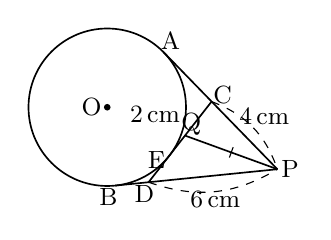
\begin{tikzpicture}[line width=0.6pt]
  \draw (0.000,0.000) circle (1.000);
  \fill (0.000,0.000) circle (1.2pt);
  \draw (2.161,-0.787) -- (0.717,0.698);
  \draw (2.161,-0.787) -- (0.101,-0.995);
  \draw (1.325,0.072) -- (0.525,-0.952);
  \draw (2.161,-0.787) -- (0.988,-0.360);
  \draw[line width=0.4pt] (1.599,-0.507) -- (1.551,-0.639);
  \node[font=\small, inner sep=1.5pt] at (0.607,-0.094) {$2\,\mathrm{cm}$};
  \draw[dashed, line width=0.4pt] (1.325,0.072) to[bend left=25] (2.161,-0.787);
  \node[font=\small, inner sep=1.5pt] at (1.994,-0.113) {$4\,\mathrm{cm}$};
  \draw[dashed, line width=0.4pt] (0.525,-0.952) to[bend right=25] (2.161,-0.787);
  \node[font=\small, inner sep=1.5pt] at (1.373,-1.168) {$6\,\mathrm{cm}$};
  \node[font=\small, inner sep=1.5pt] at (0.802,0.845) {A};
  \node[font=\small, inner sep=1.5pt] at (0.016,-1.142) {B};
  \node[font=\small, inner sep=1.5pt] at (1.464,0.152) {C};
  \node[font=\small, inner sep=1.5pt] at (0.471,-1.102) {D};
  \node[font=\small, inner sep=1.5pt] at (0.628,-0.674) {E};
  \node[font=\small, inner sep=1.5pt] at (1.068,-0.221) {Q};
  \node[font=\small, inner sep=1.5pt] at (2.321,-0.787) {P};
  \node[font=\small, inner sep=1.5pt] at (-0.200,0.000) {O};
\end{tikzpicture}
}\end{minipage}\par
